\documentclass[a4paper,11pt]{article}

\usepackage[utf8]{inputenc}

\usepackage{graphicx}
\usepackage{caption}
\usepackage{subcaption}

\usepackage{pgfplots}
\pgfplotsset{compat=1.18} 

\usepackage{minted}

\begin{document}

\title{
    \textbf{Assignment 4 Report - Sorting an array in Java}
}
\author{Dean Tsankov}
\date{\today}

\maketitle

\section*{Introduction}
In this report I will present a couple of search algorithms, every one of which has its own positives and negatives. This in turn will make it important to know when to use each according to the particular use case. In this assignment all of the work will be done with arrays of a given size and there will not be any new elements added to the data set. For each of the algorithms I will explore the run time complexity as a function of the size of the array.

\section*{Selection sort - A simple and not so efficient sort algorithm}

We begin with a simple algorithm that is not very efficient, but easy to implement, and works acceptably well with small array sizes. The general idea of the algorithm is to go through the array once and take the smallest value and put it at the beginning, next we go through the rest of the array (now without the element at the first index), find the smallest value for this sub-array and place it after the first element, shrink the sub-array where we search again and so on. Below is the provided method, filled in: 

\begin{minted}[
frame=single,
framesep=2mm,
baselinestretch=1.2,
fontsize=\footnotesize,
]{java}
    (...)
     public static void selectionSort(int[] array) {
        for (int i = 0; i < array.length - 1; i++) {
            int candidate = i;
            for (int j = i; j < array.length; j++) {
                if (array[j] < array[candidate]) {
                    candidate = j;
                }
            }
            swap(array, i, candidate);
        }
    }
    (...)
\end{minted}   

I implemented a separate {\tt swap} method, since it will also be useful in the next section.

\begin{minted}[
frame=single,
framesep=2mm,
baselinestretch=1.2,
fontsize=\footnotesize,
]{java}
    (...)
     private static void swap(int[] array, int i, int j) {
        int temp = array[i];
        array[i] = array[j];
        array[j] = temp;
    }
    (...)
\end{minted} 

Here is a plot of the benchmarks ran on this sorting algorithm:

\begin{figure}[H]
    \centering
    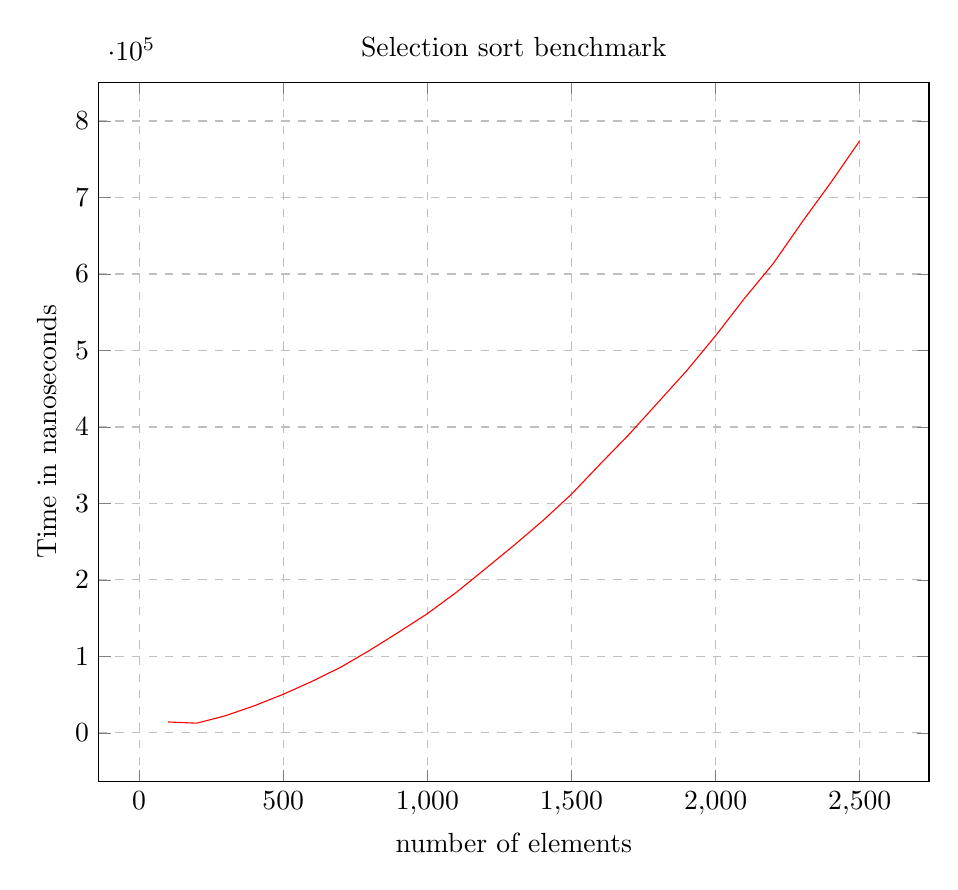
\begin{tikzpicture}
        \begin{axis}[
            title={Selection sort benchmark},
            width=\linewidth,
            xlabel={number of elements},
            ylabel={Time in nanoseconds},
            ymajorgrids=true,
            xmajorgrids=true,
            grid style=dashed,
        ]
        
        \addplot[
            color=red,
            ]
            coordinates {
            (100,14300)(200,12700)(300,22500)(400,35500)(500,50500)(600,67400)(700,86000)(800,108000)(900,131600)(1000,155900)(1100,183600)(1200,214200)(1300,245100)(1400,277300)(1500,312100)(1600,351700)(1700,390400)(1800,432000)(1900,473700)(2000,519300)(2100,568100)(2200,613700)(2300,667900)(2400,719700)(2500,774200)
            };
            
            
        \end{axis}
        \end{tikzpicture}
    \caption{Sorting over randomly generated array}
    \label{fig:plot1}
\end{figure}

We can clearly see an exponential growth considering that both axes of the graph are linearly mapped and as such we would expect the time complexity with respect to the size of the sorted over array to be {\tt O(\begin{math} n^2\end{math})}. And in fact if we think about how the algorithm works, we would come to the same conclusion, that is, if we consider the complexity as the area of our problem (since we have a nested {\tt for} loop we can view it as a 2-dimensional area) both the width and height are functions of the size n. 

Selection sort appears to perform very well if we want to quickly get, let us say, the first couple of smallest values from an array and are not interested in the rest of the data. It is, though, not a stable algorithm, meaning that if we sort data by multiple attributes, each time the previous sorting would be disregarded.

\section*{Insertion sort}

The second algorithm we are taking a look at is in some aspects similar to the first. Here instead of selecting the smallest
value, we insert the next one in the already sorted part of the array. For each value, when traversing the array, we compare it with the elements on the left side of the array, which we assume are already ordered. If the value is less we move it further back, if not we continue onto the next one in the array.
The method is simple enough to implement and makes use of the previously declared {\tt swap} function.


\begin{minted}[
frame=single,
framesep=2mm,
baselinestretch=1.2,
fontsize=\footnotesize,
]{java}
    (...)
      public static void insertionSort(int[] array) {
        for (int i = 0; i < array.length; i++) {
            int point = i;
            for (int j = i - 1; ((j > -1) && (array[point] < array[j])); 
                    j--) {
                    
                swap(array, point, j);
                point--;
            }
        }
    }
    (...)
\end{minted} 

Along with filling in the gaps of the given code I introduced a pointer index which represents the current of the sorted elements we are comparing with.

Next is this algorithm's time complexity graph, imposed onto the one for the selection sort. 

\begin{figure}[H]
    \centering
    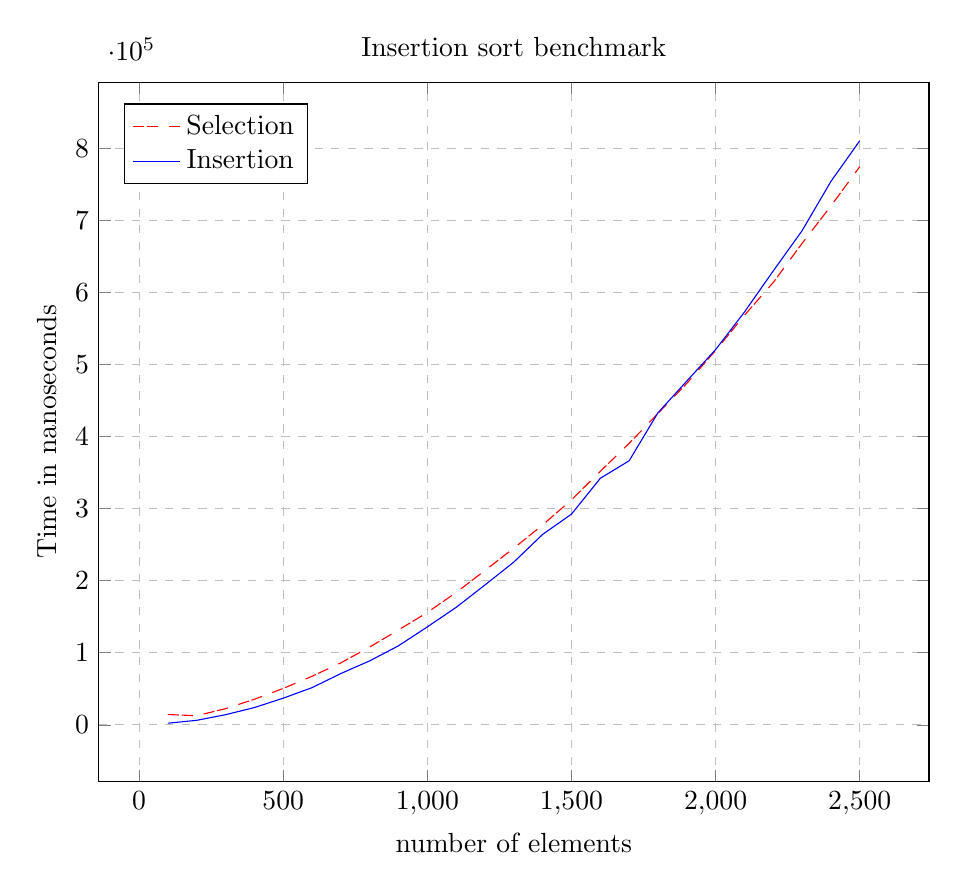
\begin{tikzpicture}
        \begin{axis}[
            title={Insertion sort benchmark},
            width=\linewidth,
            xlabel={number of elements},
            ylabel={Time in nanoseconds},
            ymajorgrids=true,
            xmajorgrids=true,
            grid style=dashed,
            legend pos=north west,
        ]
        \addplot[
            color=red,
            dash pattern=on 4pt off 1pt on 4pt off 4pt,
            ]
            coordinates {
            (100,14300)(200,12700)(300,22500)(400,35500)(500,50500)(600,67400)(700,86000)(800,108000)(900,131600)(1000,155900)(1100,183600)(1200,214200)(1300,245100)(1400,277300)(1500,312100)(1600,351700)(1700,390400)(1800,432000)(1900,473700)(2000,519300)(2100,568100)(2200,613700)(2300,667900)(2400,719700)(2500,774200)
            };
            \addlegendentry{Selection}
            
        \addplot[
            color=blue,
            ]
            coordinates {
            (100,2300)(200,6300)(300,14100)(400,24000)(500,37000)(600,51600)(700,71200)(800,88800)(900,109700)(1000,135900)(1100,163000)(1200,194100)(1300,225800)(1400,264200)(1500,292300)(1600,342000)(1700,366300)(1800,432900)(1900,476900)(2000,520500)(2100,572600)(2200,629700)(2300,685500)(2400,753800)(2500,810200)
            };
            \addlegendentry{Insertion}
            
            
        \end{axis}
        \end{tikzpicture}
    \caption{Sorting over randomly generated array}
    \label{fig:plot1}
\end{figure}

We see almost the same complexity with only slight variations. We can notice that as the problem size grows the insertion sort overtakes the selection sort gradually, meaning that it has better performance with larger n. The trade off of the two algorithms is that selection sort does more comparisons while insertion does more function calls (or generally just the swap operation). This would lead us to believe that comparison operations are generally more expensive than function calls (read/write actions) which seems to be the case.

Now insertion sort is in fact a stable algorithm, which is one advantage it has over selection sorting, but a con is the fact that it performs tremendously worse if the provided data is already sorted or semi-sorted.

\section*{Merge sort - Implementing using recursion}

Finally we will explore merge sort. The difference here is that it will require an additional array, where temporary results will be stored, before producing the final sorted array. We will also implement the algorithm recursively, that is, there will be points in the algorithm where it will call upon itself. The idea behind it goes as follows, we take the array, split it in two parts, sort each part separately and then merge both the parts together in a way which preserves the order. But how do we sort the two split parts, we call upon the same function recursively and thus split the array into even smaller parts to solve. We do this until we are left with single elements, those elements when merged into pairs will be sorted and so when we go back up the recursive stack we will end up with a sorted array. We use an auxiliary array to store the separate sorted parts of the array before merging both in the final original one.

Bellow are the 3 functions the algorithm requires to work:

\begin{minted}[
frame=single,
framesep=2mm,
baselinestretch=1.2,
fontsize=\footnotesize,
]{java}
    (...)
    public static void mergeSort(int[] org) {
        if (org.length == 0)
            return;
        int[] aux = new int[org.length];
        mergeSortSort(org, aux, 0, org.length - 1);
    }
    (...)
\end{minted}

First is the general function call which initiates the algorithm and passes the newly created auxiliary array.

\begin{minted}[
frame=single,
framesep=2mm,
baselinestretch=1.2,
fontsize=\footnotesize,
]{java}
    (...)
    private static void mergeSortSort(int[] org, int[] aux, int lo, 
            int hi) {
            
        if (lo != hi) {
            int mid = (lo + hi) / 2;
            
            mergeSortSort(org, aux, lo, mid);
            
            mergeSortSort(org, aux, mid+1, hi);
            
            mergeSortMerge(org, aux, lo, mid, hi);
        }
        return;
    }
    (...)
\end{minted}

The next method is the sorting logic i.e. the splitting of the array in depth (here the recursive call happens) and later calling the merging method.

\begin{minted}[
frame=single,
framesep=2mm,
baselinestretch=1.2,
fontsize=\footnotesize,
]{java}
    (...)
    private static void mergeSortMerge(int[] org, int[] aux, int lo, 
            int mid, int hi) {
            
        for (int i = lo ; i <= hi ; i++) {
            aux[i] = org[i];
        }
        int i = lo;
        int j = mid+1; 
        for ( int k = lo; k <= hi; k++) {
            if (i > mid) {
                org[k] = aux[j];
                j++;
            } else if (j > hi) {
                org[k] = aux[i];
                i++;
            } else if (aux[i] <= aux[j]) {
                org[k] = aux[i];
                i++;
            } else {
                org[k] = aux[j];
                j++;
            }
        }
    }
    (...)
\end{minted}

Finally the merging operation of the values stored at the auxiliary array into the original one. The logic is very simple and we just keep track of the beginnings of the two sub-arrays, compare the current two values and place the smaller into the resulting array.

Below is a graphical plot of the merge sort compared to the previous two.

\begin{figure}[H]
    \centering
    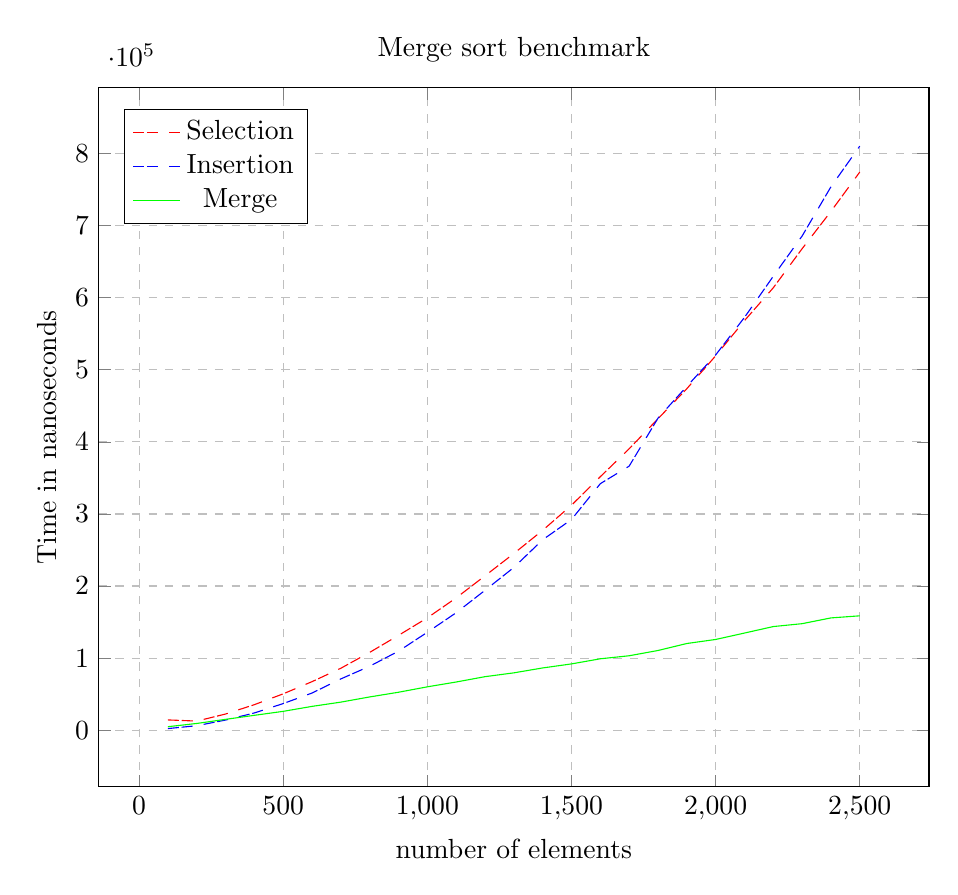
\begin{tikzpicture}
        \begin{axis}[
            title={Merge sort benchmark},
            width=\linewidth,
            xlabel={number of elements},
            ylabel={Time in nanoseconds},
            ymajorgrids=true,
            xmajorgrids=true,
            grid style=dashed,
            legend pos=north west,
        ]
        \addplot[
            color=red,
            dash pattern=on 4pt off 1pt on 4pt off 4pt,
            ]
            coordinates {
            (100,14300)(200,12700)(300,22500)(400,35500)(500,50500)(600,67400)(700,86000)(800,108000)(900,131600)(1000,155900)(1100,183600)(1200,214200)(1300,245100)(1400,277300)(1500,312100)(1600,351700)(1700,390400)(1800,432000)(1900,473700)(2000,519300)(2100,568100)(2200,613700)(2300,667900)(2400,719700)(2500,774200)
            };
            \addlegendentry{Selection}
            
        \addplot[
            color=blue,
            dash pattern=on 4pt off 1pt on 4pt off 4pt,
            ]
            coordinates {
            (100,2300)(200,6300)(300,14100)(400,24000)(500,37000)(600,51600)(700,71200)(800,88800)(900,109700)(1000,135900)(1100,163000)(1200,194100)(1300,225800)(1400,264200)(1500,292300)(1600,342000)(1700,366300)(1800,432900)(1900,476900)(2000,520500)(2100,572600)(2200,629700)(2300,685500)(2400,753800)(2500,810200)
            };
            \addlegendentry{Insertion}

        \addplot[
            color=green,
            ]
            coordinates {
            (100,4900)(200,9400)(300,15100)(400,20700)(500,26200)(600,33100)(700,39000)(800,46200)(900,52700)(1000,60200)(1100,66900)(1200,74300)(1300,79600)(1400,86400)(1500,92000)(1600,99100)(1700,103300)(1800,110600)(1900,120300)(2000,125900)(2100,134800)(2200,143800)(2300,147800)(2400,155800)(2500,158700)
            };
            \addlegendentry{Merge}
            
            
        \end{axis}
        \end{tikzpicture}
    \caption{Sorting over randomly generated array}
    \label{fig:plot1}
\end{figure}

We can see a significant reduction in time complexity. Can be equated to {\tt O(\begin{math} n*log(n)\end{math})} since for each level of the problem we are in essence splitting it in half and the complexity is taking the form of a reverse exponential function i.e. a logarithmic one. Later we have to merge all of the split parts which gives us the {\tt n} term.

Taking a look at the application of merge sort, it might be not so well suited for smaller data sets. It is also worthwhile to consider that it requires an additional supporting array. Even still it is a stable and very efficient algorithm.

\section*{Let us try to optimize merge sorting even further}

There is a very simple optimisation we can apply to our merge sort. It consists of simply moving the copying part of our merge function to the initial function call. This way we pass down two identical unsorted arrays to the {\tt MergeSortSort()} method. Then inside it, during the recursive call we toggle passing the original and auxiliary arrays. What this does is that on each level of the recursion, we are working on a separate part of either the original or aux array. Then when it comes time to merge them, all the information is already in them so there is no need to transfer anything, and we can go on comparing values and merging as before.

Here is a comparison of the optimization we implemented:

\begin{figure}[H]
    \centering
    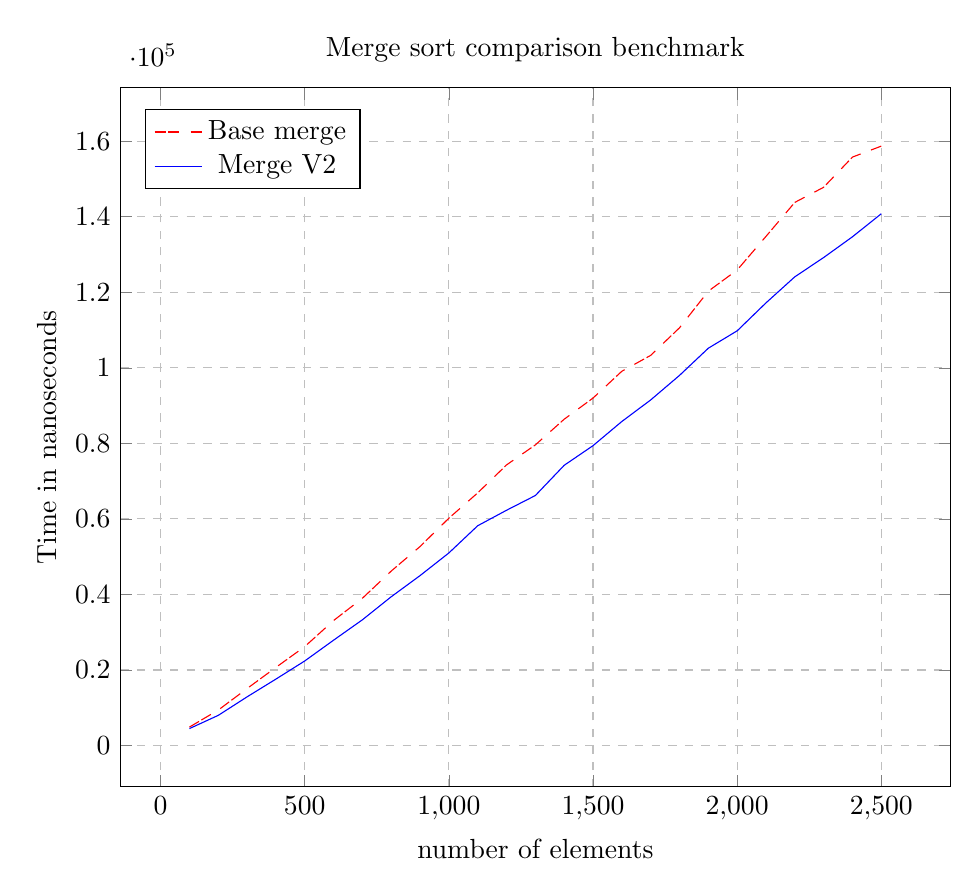
\begin{tikzpicture}
        \begin{axis}[
            title={Merge sort comparison benchmark},
            width=\linewidth,
            xlabel={number of elements},
            ylabel={Time in nanoseconds},
            ymajorgrids=true,
            xmajorgrids=true,
            grid style=dashed,
            legend pos=north west,
        ]
        \addplot[
            color=red,
            dash pattern=on 4pt off 1pt on 4pt off 4pt,
            ]
            coordinates {
            (100,4900)(200,9400)(300,15100)(400,20700)(500,26200)(600,33100)(700,39000)(800,46200)(900,52700)(1000,60200)(1100,66900)(1200,74300)(1300,79600)(1400,86400)(1500,92000)(1600,99100)(1700,103300)(1800,110600)(1900,120300)(2000,125900)(2100,134800)(2200,143800)(2300,147800)(2400,155800)(2500,158700)
            };
            \addlegendentry{Base merge}
            
        \addplot[
            color=blue,
            ]
            coordinates {
            (100,4499)(200,7999)(300,12900)(400,17600)(500,22401)(600,27900)(700,33299)(800,39399)(900,45000)(1000,50999)(1100,58200)(1200,62300)(1300,66200)(1400,74200)(1500,79400)(1600,85800)(1700,91500)(1800,98000)(1900,105199)(2000,109799)(2100,117199)(2200,124100)(2300,129200)(2400,134699)(2500,140799)
            };
            \addlegendentry{Merge V2}

            
            
        \end{axis}
        \end{tikzpicture}
    \caption{Sorting over randomly generated array}
    \label{fig:plot1}
\end{figure}

Now we definitely see there is an improvement in the execution, and if for small samples like the ones shown here the difference might seem not so significant, due to the fact that both algorithms retain their {\tt O(\begin{math} n*log(n)\end{math})} complexity, this simple alteration could prove quite beneficial.

\end{document}